%Class
\documentclass[12pt]{article}

%Package
\usepackage{multicol} 
\usepackage{graphicx}
\graphicspath{{/Users/DJYoon/Desktop/LaTex/}}
\DeclareGraphicsExtensions{.pdf,.png,.jpg,.jpeg}	


%Page
\usepackage{geometry}
\geometry{legalpaper, portrait}

%Header and Footer
\usepackage{fancyhdr}
\pagestyle{fancy}

%Title
\begin{document}
\begin{titlepage}
\begin{center}
\line(2,0){300}\\	
\huge{\bfseries Head Scope} \\
\textsc{\large Application for Head Mounted Display}\\[2\baselineskip]
\end{center} 

%HYU Image
\center

\includegraphics{TeamName}
\\ [9\baselineskip]


%Taehun(Top Left) 

\begin{multicols}{2} \noindent 
\textsc {\noindent TaeHun Kim\\ 
Information System in HYU \\
 2011004426 \\ 
 chutbaksa@gmail.com}\\[1\baselineskip]
%SeungSun(Bottom Left)
\textsc{SeungSeon Shin \\
 Information System in HYU 
 \\ 2011004512 \\ 
 vgb1873@gmail.com}\\[1\baselineskip]
%DukJin (Top Right)			
\textsc{Duk Jin Yoon \\
Information System in HYU \\
2011004534 \\
yoondukjin@outlook.com} \\[1\baselineskip]
%Seung Gyu (Bottom Right)
\textsc{Seunggyu Jin \\ 
Information System in HYU \\
2013012740 \\
bernardjin@naver.com}
\end{multicols}
\end{titlepage}



%Table of Contents
\tableofcontents
\pagenumbering{roman}
\cleardoublepage
%\addcontentsline{toc}{section}{\numberline{}Test}


%Table
\section*{Role Assignment}
{\footnotesize \noindent \textit {Keywords - Head Mounted, Telepresence, Virtual Reality, Google Cardboard }}\\
\begin{table}[htb]
\centering
\caption[Role Assignment]{Role Assignment}
\begin{tabular}{|c|c|p{6cm}|}
\hline
\textbf{Roles}& \textbf{Name} & \textbf{Task Description and Etc.}\\ \hline

User & Kim & Assuming himself as a software user.
Discuss about softwares weak point, strong point.\\ \hline

Customer & Shin & Discuss about whole financial costs. \\ \hline

Software Developer & Yoon & Develop entire software. Consider about the program.\\ \hline

Developer manager & Jin & Lay out our rough sketch. Managing our plan.\\ \hline

\end{tabular}
\end{table}


%Abstract
\pagenumbering{arabic}
\setcounter{page}{1}
\section{Abstract}

Screen displays are primarily advancing to a sharper resolution with larger screens to increase the satisfaction of the consumers. However, in spite of all the upgraded specifications, screen displays still remains as a frame. It is a frame that will only let us view the other world; and we wanted to change this view. Our team wanted to let the viewers to be inside the other world. This principal is called, Virtual Reality. With VR(Virtual Reality), we are able to let users to feel the present in the other world. Our team will implement the VR through Google Cardboard and an Android Smartphone. The Google Cardboard will be used as a viewing tool with asymmetric biconvex lenses, and the Smartphone will be used as a display screen with an application that creates a 3D reality when viewed through the Google Cardboard.\\





%Introduction
\section{Introduction}

Films. Film is an incredible medium that is designed with a group of rectangle pictures that are played in a sequence. Though these pictures it can tell us stories in different ways. Film is like a window that lets you see the other world. However, our team wanted something else, we wanted something that allows you to be in the other world. It is called Virtual Reality.  Virtual Reality is a machine. But through this machine it allows us to have access to another world and feel present in the world that you are inside. Our team will use the Google Cardboard, which is a box built in the shape of a snorkeling glass. Inside this Google Cardboard there are two lenses that are made of asymmetric biconvex lenses that allows one to experience a 3D reality. Along with the Google Cardboard, we will insert an android smartphone in the form of landscape and build an application that will change 2D to 3D. Inside this application we will install two functions GoogleMap and Cinema Film.   Inside this Google Cardboard, it will let you feel like it is real life, and let you feel the presence of the people you are with. That is why we we chose GoogleMap and Cinema Film. With GoogleMap, it allows users to experience a full 360-degree view of the designated location. It will give them a detailed view and feel as if they are in that location. The Cinema Film will be built so that it allows the users to feel as if they were in the presence of the film.   With Google Cardboard, it will let us see not a view into the world, but the whole world stretched in a rectangle. It is a form of media that can change peoples perception of each other. Our team believes that Virtual Reality has the potential that can change the world. We become more empathetic, and we become more connected. Ultimately, we become more human.

%Requirement
%Section
\section{Requirement}
%Subsection 1
\subsection {Requirement for Head Mounted Display}

%Subsubsection 1
\subsubsection{Overview}
A typical HMD has either one or two small displays with lenses and semi-transparent mirrors embedded in a helmet, eyeglasses or visor.

\subsubsection{Google CardBoard}

\begin{itemize}
\item We will use Google Cardboard for several reasons.
\item Google Cardboard is relatively cheaper than other HMD.
\item Google Cardboard could use smart phones gyroscope function.(Because some display machines could not use gyroscope function.)
\item Google Cardboard has very powerful accessibility. It has very reasonable price, and many people can use it without a big burden.
\end{itemize}

\subsubsection{Input Device}
\begin{enumerate}
\item Magnetic Pull
\item Smartphone within gyroscope
\end{enumerate}

\subsubsection{Output Device}
\begin{enumerate}
\item Smartphone (Audio and Screen)
\item Show Screen through Head Mounted Display
\end{enumerate}

\subsubsection{Requirement for Application Logo}
\begin{enumerate}
\item We will design our application logo, using Adobe Photoshop CS6 and Adobe Illustrator CS6.
\item Display it on the Smartphone.
\end{enumerate}

\subsubsection{Requirement for loading page}
\begin{enumerate}
\item Show our application name
\item Show our team name
\end{enumerate}

\subsubsection{Requirement for main page}
\begin{enumerate}
\item It would have four item
\item Jumper (Telepresence to Google Earth API)
\item Cine (Telepresence movie viewer)
\end{enumerate}

\subsubsection{Requirement for Jumper}
\begin{enumerate}
\item Click the Jumper Icon among the main page
\item Show the photographs of tourist attraction on the wall
\item To use gyroscope, users will  find the photograph which they want to go
\item Users will choose the photograph by pulling down the Magnetic pulling
\item Users are able to trip the attraction zone
\item If the tour is over, users could exit by back button
\end{enumerate}

\subsubsection{Requirement for Cine}
\begin{enumerate}
\item Click the Cine Icon among the main page
\item Show the movie poster on the notice board
\item To use gyroscope and Magnetic button, users will find the movie which they want to see and choose the movie
\item Users could be able to watch the movie to have experience the ambience of a movie theater
\item If the movie is over, users could exit by back button
\end{enumerate}

%Subsection 2
\subsection{Development Environment}
Before you begin to format your paper, first write and save the content as a separate text file. Keep your text and graphic files separate until after the text has been formatted and styled. Do not use hard tabs, and limit use of hard returns to only one return at the end of a paragraph. Do not add any kind of pagination anywhere in the paper. Do not number text heads-the template will do that for you.
Finally, complete content and organizational editing before formatting. Please take note of the following items when proofreading spelling and grammar:

%subsubsection 2

\subsubsection{Choice of software development platform}
\begin{enumerate}
\item Which platform and why. We will use Windows, Yosemite for android application development.
\item Which  program language and why. We will use Java(Cardboard SDK for Android) for internal functions. We also use XML for design layouts. We will use Unity for 3D Modeling.
\item Provide a cost estimation for your built. We need Photoshop CS6 WON 323,158  but we think it is so expensive so we use trial version of Photoshop for free. Next, we need Google Cardboard. We can buy it WON 5,000.\\ \\
Android develop\\
Windows7 ultimate\\
OS X Yosemite 10.10.2\\
Android Studio\\
Adobe Photoshop CS6 trial version\\
Unity 5 Engine\\
\end{enumerate}

\subsubsection{Software in Use}
\begin{enumerate}
\item There is already a Google Cardboard application that is built by Google.
\end{enumerate}

%subsection 3

\subsection{Specification}

%subsubsection 3

\subsubsection{Specification of App Icon}
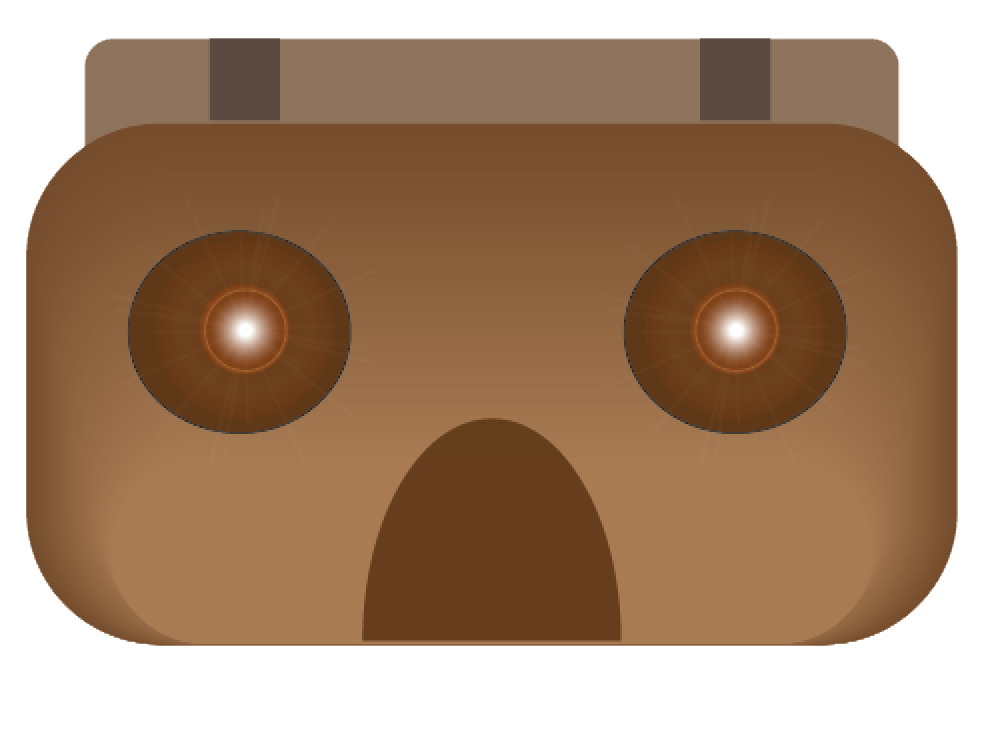
\includegraphics[width=50mm,scale=0.5]{HeadScope_APP}

%subsubsection 4
\subsubsection{Specification of Loading App Page}

\newpage
\subsubsection{Specification of Main App Page}

\includegraphics{Main}
\begin{enumerate}
\item The Main App Page would have five applications:\\ \\
 Jumper\\
 3D Cube\\
 Volume\\
 Preferences\\
 Exit\\
\item Due to the gyroscope sensor built in the smartphone, we are able to select different apps inside the Main App Page by turning your head. We built a fixed cursor that will guide the users to what they are selecting. To select the desired app, users will simply pull down the magnetic pull.
\end{enumerate}

%subsubsection 5
\subsubsection{Specification of Jumper}
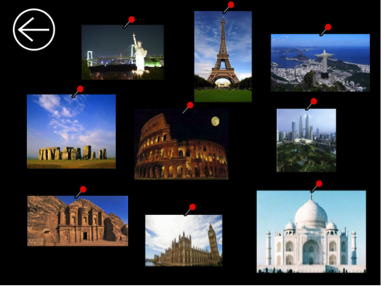
\includegraphics{Jumper}

\begin{enumerate}
\item The Jumper application will allow users to view an image in a 360 degree angle. This will give them a full view from the side to the back of an image by turning their head around. Jumper can give the users the experience to actually feel like their in that place. 
\item By using gyroscope, users will find the attraction place which they want to go and will choose the photograph.\\
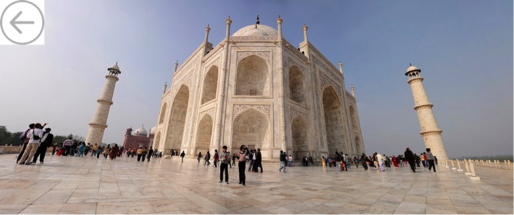
\includegraphics{View}
\item Since the image needs to be 360 degrees there are a limited number of images that we will be implementing. In addition, users are unable to upload their own image. However, our team will continue to update pictures from the famous attraction places such as: Namsan, Eiffel Tower, and even Egypt's Pyramids.
\end{enumerate}

%subsubsection 6
\subsubsection{Specification of 3D Cube}
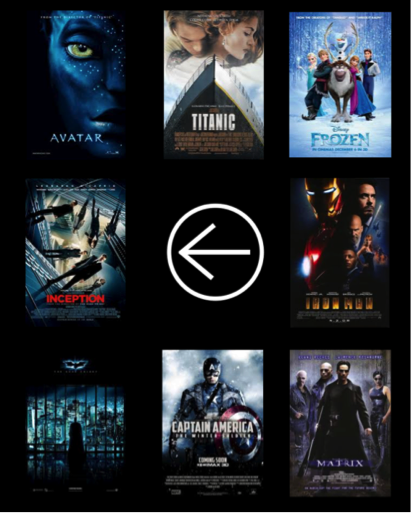
\includegraphics{Cine}

\begin{enumerate}
\item Upon clicking the 3D Cube App icon, users will search for the moving 3D Cube object. 
\item After the user find the 3D Cube, the users will lower the magnetic button that is installed in the Google Cardboard.
\item This will change the 3D Cube's color.
\item There is a point system within the app that counts the number of times the user find the 3D Cube object.
\end{enumerate}

%subsubsection 7
\subsubsection{Specification of Volume}

%includegraphics{} <-- image of the Volume icon

\begin{enumerate}
\item The Volume icon will adjust the amplification of the HeadScope application. 
\item Users are able to adjust the volume by turning their head towards the left for a lower sound and to right for a louder sound.
\end{enumerate}

%subsubsection 8
\subsubsection{Specification of Preferences}

%includegraphics{} <-- image of the Preference icon

\begin{enumerate}
\item The Preferences App Icon will display the settings based on the HeadScope App.
\item The first setting have a checkbox for smartphones that do not work with the magnetic pull. For those users whom smartphones do not support the Google Cardboards magnetic pull, there is an alternative. Users are able to select apps by holding the cursor shown in the smartphone steadily. Once the users hold the smartphone steadily there will be circle cursor that will fill when not moved. As soon as the circle is filled, the smartphone will select that app.
\item The second setting will contain a checkbox that makes the VR experience more seamless. This can create a smooth transition between apps without exiting the application.
\item The third setting is a function that allows the list of apps to be separated by commas, that the launcher will display.
\item The fourth setting has the same function of the third, but in a blacklist.
\item The fifth setting is the adjustment for the Interpupillary Distance. This setting is the distance between your pupils. 0 is set for pupils that are very
close and 100 for pupils that are far apart.
\item The sixth setting is a checkbox for users to disable vibration when selecting an app. When enabled, the phone will initiate a vibration upon selecting a desired application.
\item The seventh setting is a checkbox that will disable the volume buttons in the smartphone. Users will sometime experience situations where they accidentally press their smartphones volume button. For this case, we implemented an override method to disable the volume button when the HeadScope application is running.
\item The eight setting is premium checkbox that when clicked it will give direct users to our teams homepage. This is made just for users to donate to our project.
\item The ninth setting is a checkbox that allows users to modify the Main App Pages background. If not checked the Main App Page will have a default background which is the color of black.
\item The last setting is a checkbox that allows the voice recognition command. To launch the apps in the Main App Page users can also use the smartphones integrated voice command. This is an alternative choice for selecting apps instead of the magnetic pull.
 
 
\end{enumerate}

\end{document}

